%%%%%%%%%%%%%%%%%%%%%%%%%%%%%%%%%%%%%%%%%
% Short Sectioned Assignment
% LaTeX Template
% Version 1.0 (5/5/12)
%
% This template has been downloaded from:
% http://www.LaTeXTemplates.com
%
% Original author:
% Frits Wenneker (http://www.howtotex.com)
%
% License:
% CC BY-NC-SA 3.0 (http://creativecommons.org/licenses/by-nc-sa/3.0/)
%
%%%%%%%%%%%%%%%%%%%%%%%%%%%%%%%%%%%%%%%%%

%----------------------------------------------------------------------------------------
%	PACKAGES AND OTHER DOCUMENT CONFIGURATIONS
%----------------------------------------------------------------------------------------

\documentclass[paper=a4, fontsize=12pt, toc=left]{scrartcl} % A4 paper and 11pt font size
\usepackage[letterpaper,margin=1in]{geometry}

\usepackage[hidelinks]{hyperref}
\usepackage[T1]{fontenc} % Use 8-bit encoding that has 256 glyphs
%\usepackage{fourier} % Use the Adobe Utopia font for the document - comment this line to return to the LaTeX default
\usepackage{libertine}
\usepackage[english]{babel} % English language/hyphenation
\usepackage{amsmath,amsfonts,amsthm} % Math packages

\usepackage{lipsum} % Used for inserting dummy 'Lorem ipsum' text into the template

\usepackage{sectsty} % Allows customizing section commands
%\allsectionsfont{\centering \normalfont\scshape} % Make all sections centered, the default font and small caps
\allsectionsfont{\centering \normalfont} % Make all sections centered, the default font

\usepackage{fancyhdr} % Custom headers and footers
\pagestyle{fancyplain} % Makes all pages in the document conform to the custom headers and footers
\fancyhead{} % No page header - if you want one, create it in the same way as the footers below
\fancyfoot[L]{} % Empty left footer
\fancyfoot[C]{} % Empty center footer
\fancyfoot[R]{\thepage} % Page numbering for right footer
\renewcommand{\headrulewidth}{0pt} % Remove header underlines
\renewcommand{\footrulewidth}{0pt} % Remove footer underlines
\setlength{\headheight}{13.6pt} % Customize the height of the header

\numberwithin{equation}{section} % Number equations within sections (i.e. 1.1, 1.2, 2.1, 2.2 instead of 1, 2, 3, 4)
\numberwithin{figure}{section} % Number figures within sections (i.e. 1.1, 1.2, 2.1, 2.2 instead of 1, 2, 3, 4)
\numberwithin{table}{section} % Number tables within sections (i.e. 1.1, 1.2, 2.1, 2.2 instead of 1, 2, 3, 4)

%\setlength\parindent{0pt} % Removes all indentation from paragraphs - comment this line for an assignment with lots of text

%----------------------------------------------------------------------------------------
%	TITLE SECTION
%----------------------------------------------------------------------------------------

\newcommand{\horrule}[1]{\rule{\linewidth}{#1}} % Create horizontal rule command with 1 argument of height

\title{	
\normalfont \normalsize 
\textsc{TECHNOTE} \\ [25pt] % Your university, school and/or department name(s)
\horrule{0.5pt} \\[0.4cm] % Thin top horizontal rule
\huge Neutron Production by Cosmic Ray Muons \\ % The assignment title
\horrule{2pt} \\[0.5cm] % Thick bottom horizontal rule
}

\author{Shih-Kai Lin \\
University of Houston \\
email: \small\texttt{slin8@uh.edu}} % Your name

\date{\normalsize\today} % Today's date or a custom date


%--------------------------------------------------------
% Infile References
%--------------------------------------------------------
\usepackage[style=numeric,sorting=none,backend=bibtex]{biblatex}
\bibliography{references}
%\begin{filecontents}{references.bib}
%@ARTICLE{docdb6759,
%    AUTHOR={Jiajie Ling and Haoqi Lu},
%    TITLE={Muon Tagging},
%    JOURNAL={DocDB-6759}
%}
%\end{filecontents}



\begin{document}

\maketitle % Print the title
\pdfbookmark{\contentsname}{toc}
\tableofcontents
\newpage

%----------------------------------------------------------------------------------------
%	Introduction talking about motivation
%----------------------------------------------------------------------------------------

\section{Goal}

In this document we describe in detail how neutron yield is measured and compare it to results from other literature.


%------------------------------------------------

\section{Methodology}
We propose a data-driven geometric method to account for the neutron spill-in/spill-out effects which can be compared with a full neutron Monte Carlo simulation once it is available.

Neutron yield is the number of neutrons produced by a muon when it traverses a unit length of the material. In this study we are interested in the neutrons produced in the target material, GdLS. The GdLS not only serves as the target but also serves as the neutron detector. Once a induced neutron is captured on Gd, the neutron position can be reconstructed within a 20 cm resolution~\cite{docdb7334}. In Daya Bay's experimental halls, muons come in at all angles and penetrate the inner acrylic vessel (IAV) from all points and angles. Assuming the neutron capture position is axially symmetric around the muon track, a symmetric fiducial volume can be constructed around the track fully enclosed in the GdLS. This way we can decompose the neutron capture position into its axial and lateral components and apply symmetry arguments to account for the spill-in/spill-out effects.

\begin{figure}[h]
	\centering
	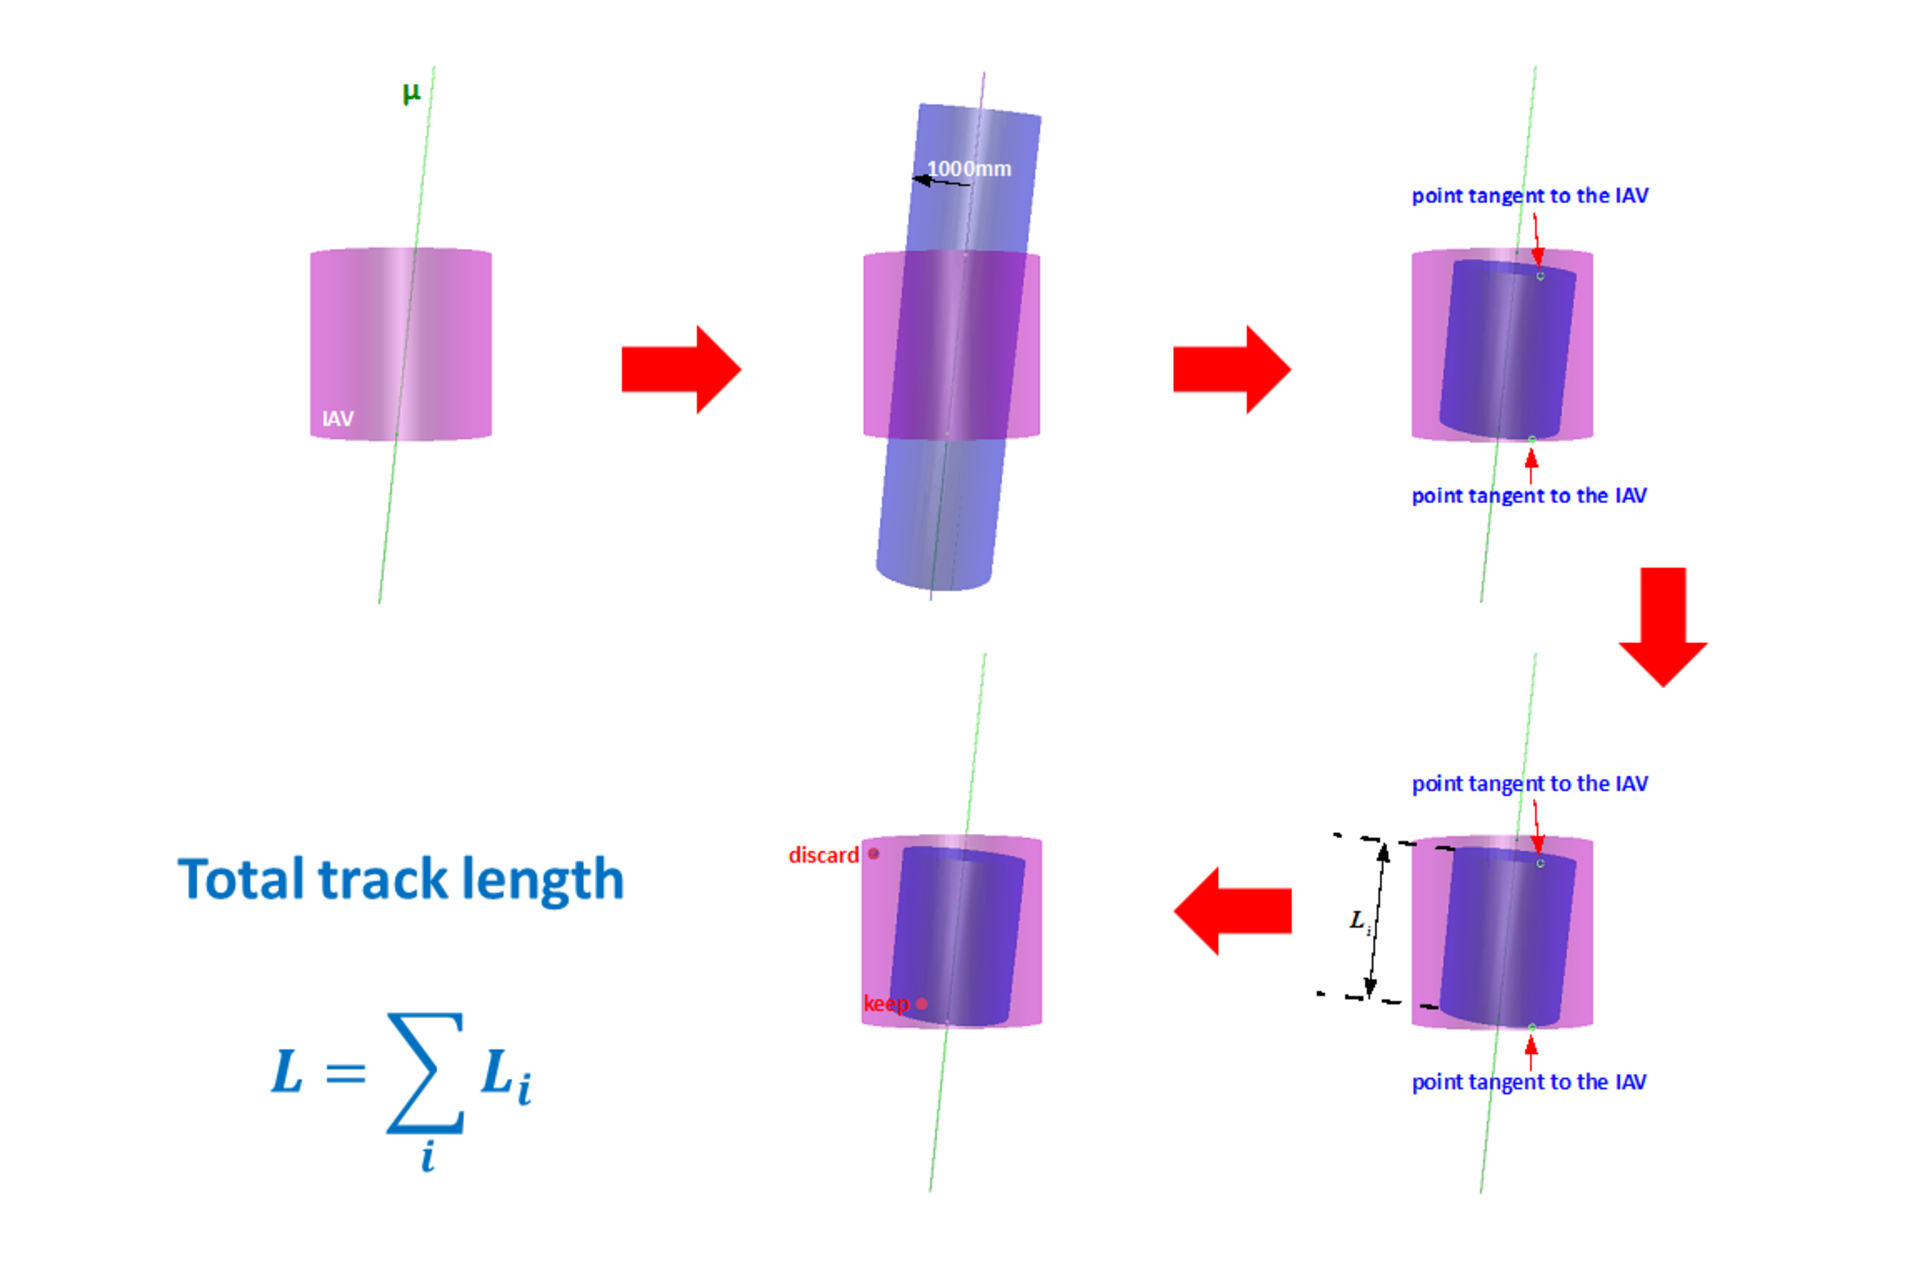
\includegraphics[width=\textwidth]{figures/fiducial_illustration.eps}
	\caption{A cartoon showing how a symmetric fiducial volume is constructed.}
	\label{fig:fiducial_illustration}
\end{figure}
Figure~\ref{fig:fiducial_illustration} shows how a symmetric fiducial volume can be constructed given a reconstructed muon track. This problem can be solved exactly numerically and details can be found in~\ref{app:a}. After constructing the fiducial volume, the height of the inscribed fiducial cylinder is taken as the muon track length. Only neutrons captured within the fiducial cylinder are kept.


\section{Event Selection}

\subsection{Muon Selection}

Since a muon can traverse multiple detectors at a time, a muon is actually identified as a group of muon triggers across detectors in data.

The muon selection starts with muon triggers grouped in the directory \scriptsize\path{/Event/Data/Physics/Spallation} \normalsize in production files. The grouping first identifies whether a trigger satisfies the MuonAny criteria. MuonAny is the loosest muon tag which includes all triggers with IWS NHIT > 6 or OWS NHIT > 8 or AD charge > 3000 pe or RPC 3/4 or 4/4 layers being fired (i.e., excluding the RPC forced triggers). Then all MuonAny triggers have to be within 300 ns after the first MuonAny trigger to form the so called MuonPrompt triggers which completes the muon grouping process. For more details, see Ref.~\cite{docdb6759} . In order to reconstruct a muon track, a valid OWS reconstructed point with PoolSinple algorithm and a valid RPC reconstructed point with RpcSimple algorithm are required. Note that requiring a valid RPC point will rule out RPC forced triggers automatically. Finally, in order to apply the fiducial cut, only tracks around which a fiducial cylinder with radius 1000 mm can fit in the IAV are kept.

\vspace{\baselineskip}
To summarize the muon selection criteria,
\begin{itemize}
  \item satisfies MuonAny criteria:
        \\IWS NHIT > 6 or OWS NHIT > 8 or AD charge > 3000 pe or RPC 3/4 trigger
  \item all MuonAny triggers within 300 ns since the first MuonAny trigger
  \item valid points with PoolSinple and RpcSimple so that a track is formed by two points connection
  \item tracks around which a cylinder with 1000 mm can fit in the IAV
\end{itemize}

\subsection{Neutron Selection}

Neutron selection at this point is more straightforward. The neutron has to be Gd captured and within the fiducial volume. A Gd captured neutron is identified with its energy and timing. Here we use IBD neutron energy cut, 6 MeV < $E_n$ < 12 MeV. For the timing cut we first choose the upper bound at 1000 $\mu$s after the muon which could be fine tuned and optimized with ease. The lower bound is set at 20 $\mu$s after the muon to avoid PMT ringing and AD retriggers. Also a flasher cut is applied to ensure the event is physical.

\vspace{\baselineskip}
To summarize the neutron selection criteria,
\begin{itemize}
  \item 6 MeV < $E_n$ < 12 MeV
  \item 20 $\mu$s < $t_n-t_\mu$ < 1000 $\mu$s
  \item within the fiducial volume constructed in muon selection
  \item non-flasher event
\end{itemize}


\section{Neutron Yield}
Measuring the neutron yield is closely related to measuring the muon-nucleus total interaction cross section since the number of neutrons produced can be written as
\begin{equation} \label{eq:neutron_number}
	\bar{N}_n=n\left\langle\nu\sigma\right\rangle\ell=\frac{\rho N_A}{A}\left\langle\nu\sigma\right\rangle\ell
\end{equation}
where $\bar{N}_n$ is the mean number of neutrons produced per muon, $n$ is the number density of the medium the muon traverses, $\nu$ is the neutron multiplicity per interaction, $\sigma$ is the muon-nucleus total interaction cross section, $\ell$ is the mean track length of the muon, $\rho$ is the mass density of the medium, $N_A$ is the Avogadro number and $A$ is the atomic mass of the medium. Because muons could interact with different nucleus in the medium and produce different number of neutrons, the mean value of the product $\left\langle\nu\sigma\right\rangle$ is used.

Experimentally the neutron yield is given by
\begin{equation} \label{eq:ideal_neutron_yield}
	Y_n=\frac{\bar{N}_n}{\ell\rho}=\frac{N_n}{L\rho}
\end{equation}
where $Y_n$ is the neutron yield, $N_n$ is the total number of neutrons produced by all muons and $L$ is the total muon track length traversed by all muons.

From Eq.~\ref{eq:neutron_number} and Eq.~\ref{eq:ideal_neutron_yield} the mean value of the product of the neutron multiplicity and the muon-nucleus total interaction cross section is
\begin{equation}
	\left\langle\nu\sigma\right\rangle=\frac{Y_nA}{N_A}
\end{equation}

However since 100\% neutron detection efficiency can not be achieved experimentally due to the neutron selection cuts and finite detector acceptance, the produced number of neutrons is estimated by $N_n^s/\epsilon$, the number of selected neutrons corrected by the total selection efficiency, which is a product of several efficiency terms. In this study,
\begin{equation}
	\epsilon=\epsilon_{Gd}\epsilon_E\epsilon_T\epsilon_{acc}
\end{equation}
where $\epsilon_{Gd}$ is the Gd capture ratio, $\epsilon_E$ is the energy cut efficiency, $\epsilon_T$ is the timing cut efficiency and $\epsilon_{acc}$ is the detector acceptance due to the fiducial cut.

The yield formula used in this study is then
\begin{equation}
	\boxed{Y_n=\frac{N_n^s}{\epsilon_{Gd}\epsilon_E\epsilon_T\epsilon_{acc}L\rho}}
\end{equation}

Since the muon-nucleus total interaction cross section depends on the muon energy, the neutron yield also does. The pioneering work was done in 1965 by G. T. Zatsepin and O. G. Ryazhskaya~\cite{Zatsepin1965} who proposed the yield to follow a simple power law,
\begin{equation}
  \boxed{Y_n(\bar{E}_\mu)=\alpha\bar{E}_\mu^\beta}
\end{equation}
where $\bar{E}_\mu$ is the mean muon energy and $\alpha$ and $\beta$ are parameters to be fitted with data. This formula is largely confirmed by FLUKA and GEANT4 simulations~\cite{Wang2001}~\cite{Araujo2005}~\cite{Mei2006}~\cite{Malgin2008} as well as by measurements~\cite{Gorshkov1971}~\cite{Bezrukov1973}~\cite{Enikeev1987}~\cite{Aglietta1989}. However large tensions in the values of $\alpha$ and $\beta$ still remain. The Daya Bay experiment has three experimental halls each with different overburden. In principle Daya Bay, a single experiment, can measure three yield values corresponding to three different mean muon energies.

There are therefore 8 terms to be determined in order to measure the yield as a function of the mean muon energy, namely $N_n^s$, $\epsilon_{Gd}$, $\epsilon_E$, $\epsilon_T$, $\epsilon_{acc}$, $L$, $\rho$ and $\bar{E}_\mu$. In the following sections each term and its uncertainty will be discussed in detail.

The discussion will start with more widely studied quantities and move on to the quantities more specific to this study.

\subsection{Gd Capture Ratio \texorpdfstring{$\epsilon_{Gd}$}{epsilon Gd}}
Spallation neutrons generated in the target mass, GdLS, may not all be captured on Gd. Some could be captured on H or other nuclei. Some are not captured at all and leave the detector which we call spill-out neutrons. There are also spill-in neutrons, namely neutrons generated outside and transport into the target mass and get captured on Gd. Since in this study we select only the Gd captured neutrons, we have to determine this efficiency which is often called the Gd capture ratio.

Many studies had been done on the Gd capture ratio with spallation neutrons~\cite{docdb7273}~\cite{docdb7524}~\cite{docdb7525}, calibration sources~\cite{docdb7273}~\cite{docdb7525}, special calibration runs~\cite{docdb8280}~\cite{docdb8473}~\cite{docdb8501}~\cite{docdb9226}~\cite{docdb9273} and Monte Carlo simulation~\cite{docdb7730}. However different studies adopt slightly different definitions of this ratio. Here we define the Gd capture ratio as
\begin{equation} \label{eq:gd_capture_ratio}
	\epsilon_{Gd}=\frac{\text{number of neutrons generated in GdLS and captured on Gd}}{\text{number of neutrons generated in GdLS}}
\end{equation}

We use the more up-to-date study by Gaosong~\cite{docdb9273}. In Gaosong's study a complete comparison between AmC, AmBe, PuC and Monte Carlo is given and the efficiency due to energy cuts is corrected for resulting in a $\epsilon_{Gd}$ definition which coincides with Eq.~\ref{eq:gd_capture_ratio}. A final result is quoted as,
\begin{equation}
  \epsilon_{Gd}=85.2\%\pm 0.4\%
\end{equation}


\subsection{Energy Cut Efficiency \texorpdfstring{$\epsilon_{E}$}{epsilon E}}

One of the signature of a neutron captured on Gd is the 8 MeV $\gamma$ energy released from the de-excitation of Gd*. Once a neutron is captured on Gd, the 8 MeV $\gamma$'s result regardless of the initial energy and momentum of the neutron. Therefore we use the 8 MeV energy cut efficiency published in the IBD analysis~\cite{dayabay2012_1}, combining the correlated and uncorrelated uncertainties,
\begin{equation}
	\epsilon_{E}=90.9\%\pm 0.61\%
\end{equation}


\subsection{Capture Time Cut Efficiency \texorpdfstring{$\epsilon_{T}$}{epsilon T}}

The other signature of a neutron captured on Gd is the capture time whose mean value is $\sim 28\mu s$. Figure~\ref{fig:IBD_capture_time} shows the IBD neutron capture time distribution. The distribution is not a simple exponential but has a rising edge in the beginning of the spectrum. Xin and Chao proposed a 2-exponential fit to model the whole spectrum~\cite{docdb7299}, one of which accounts for the rising edge due to the thermalization of neutrons.
\begin{figure}
	\centering
	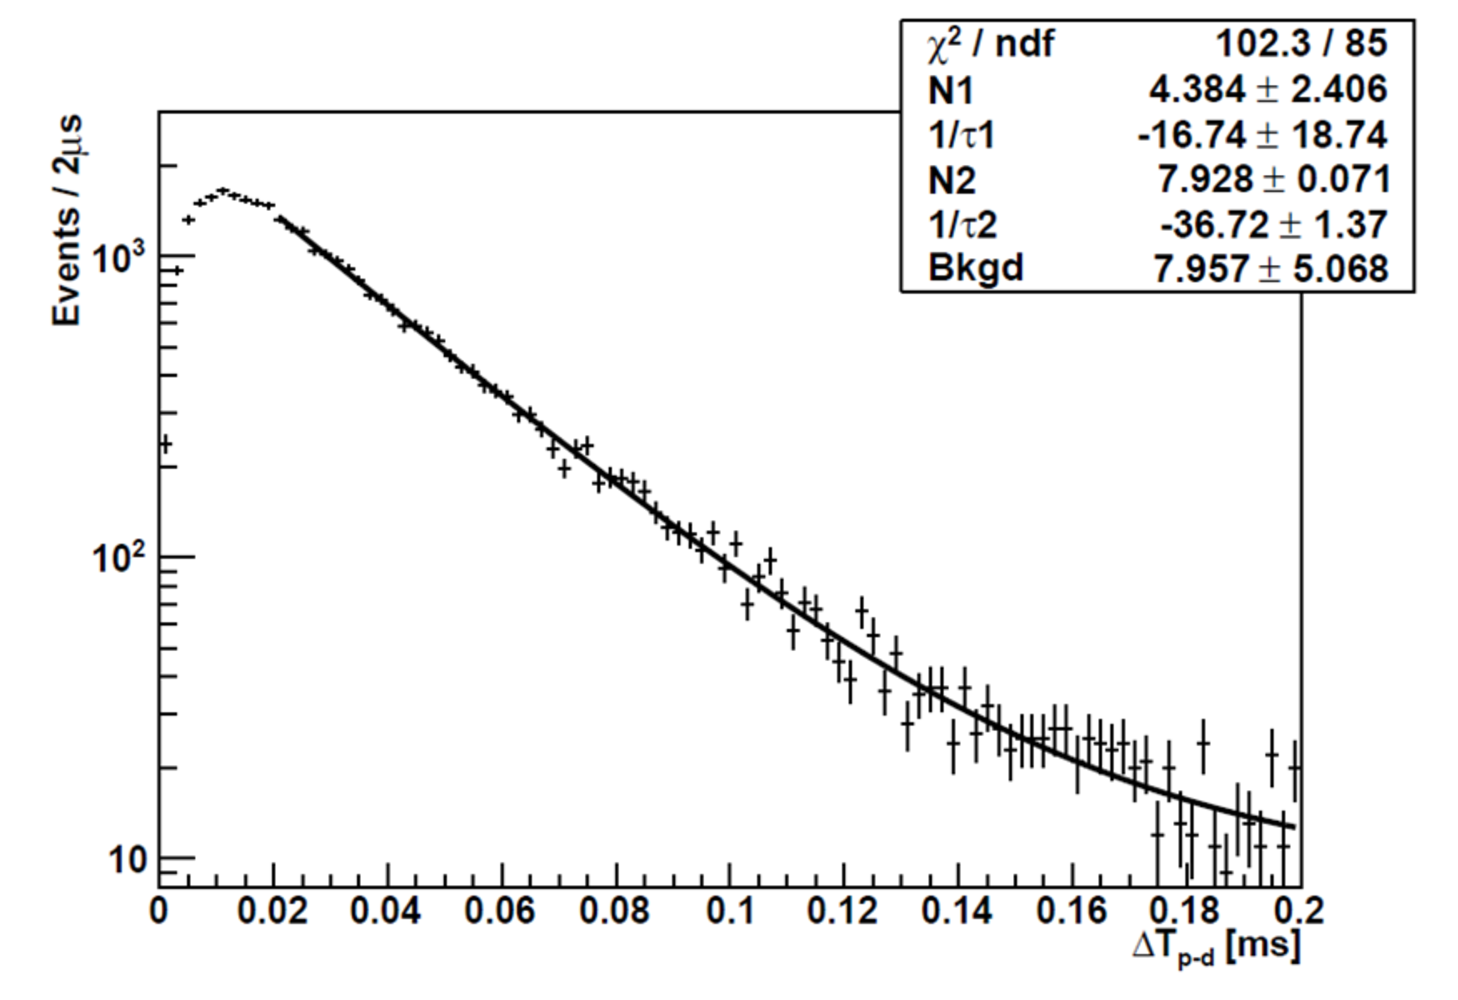
\includegraphics[width=.6\textwidth]{figures/IBD_capture_time.eps}
	\caption{IBD neutron capture time distribution~\cite{docdb7299}}
	\label{fig:IBD_capture_time}
\end{figure}


%%%%%%%%%%%%%%%%%%%%%%%%%%%%%%%%%%%%%%%%%%%%%%%%%%%%%%%%%
% Appendix About How the Fiducial Volume Is Constructed
%%%%%%%%%%%%%%%%%%%%%%%%%%%%%%%%%%%%%%%%%%%%%%%%%%%%%%%%%

\appendix
\gdef\thesection{Appendix \Alph{section}}
\section{Constructing the Fiducial Volume} \label{app:a}
We start with a IAV cylinder whose radius is $R$ and height is $H$. A straight line goes through this cylinder. The problem is to find a cylinder with a given radius $r<R$ coaxial with the straight line which is fully enclosed in the IAV cylinder. Of course, if a fiducial cylinder with height $h$ is a solution, any coaxial cylinder with height $h'<h$ and share the same center is also a solution. Note here we call the midpoint on the axis between the top and bottom of the cylinder the cylinder center. We want to find the maximum value of $h$.

The starting point is to elongate the two cylinders to infinity and look at how they intersect.


\printbibliography[heading=bibintoc]

\end{document}